\begin{task}
\textbf{Задача 10. }Привести пример функции $f: \mathbb{R} \rightarrow \mathbb{R}$, всюду дифференцируемой по Фреше, но не строго дифференцируемой в нуле.

\textbf{Доказательство:}
Рассмотрим функцию $f$:
\[
f(x)= \begin{cases}0, & x=0 \\ x^2 \sin \left(\frac{1}{x}\right), & x \neq 0\end{cases} 
\]

\begin{figure}[h!]
\centering
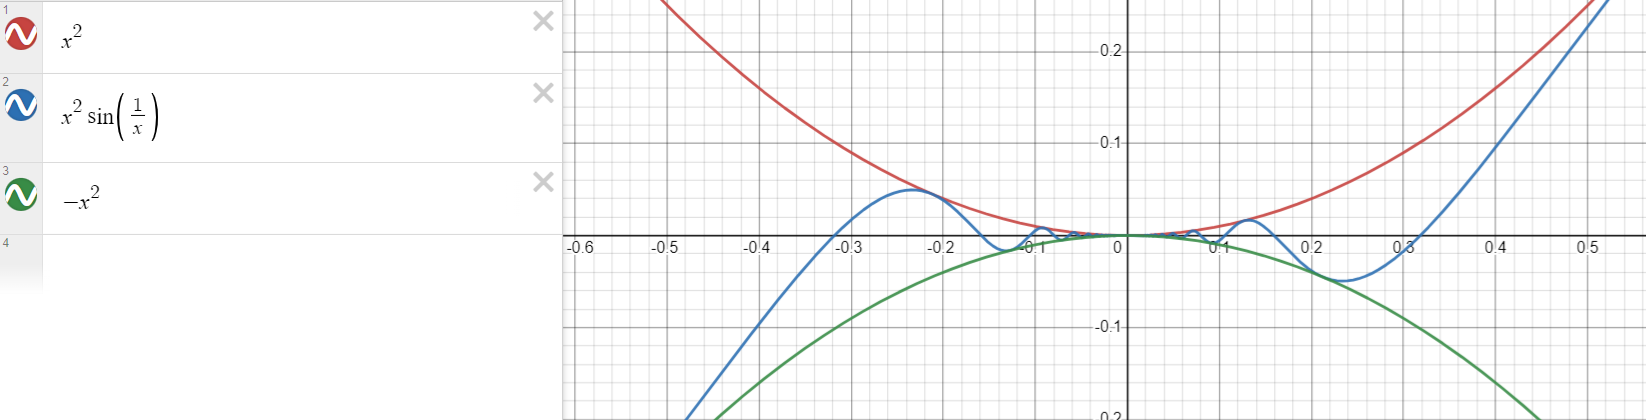
\includegraphics[width=0.99\linewidth]{image.png}
\end{figure}
 
$f$ дифференцируема по Фреше в $x \neq 0$ (по правилу Лейбница):
\[\begin{aligned}
&(x+h)^2 = x^2 +2xh+ \bar{o}(|h|)\\
& \sin{\frac{1}{x+h}} = \sin{\frac{1}{x}} + \frac{-1}{x^2} \cos{\frac{1}{x}}h + \bar{o}(|h|)
\end{aligned}\]
$|f(x)| \leq x^2 \implies f^{\prime}(0)=0$ и $f(x)-f(0)=f(x) =\bar{o}(|x|), |x| \rightarrow 0 $
то есть f диф. по Фреше в 0, тогда и на всем $\mathbb{R}$

Предположим противное: $f$ строго дифференцируемо в $0$.

По определению,  для любого $\varepsilon>0$ существует $\delta>0$ такое, что для любых $x_1, x_2 \in O_\delta\left(x_0\right)$ выполнено
\[\begin{aligned}
&|f\left(x_1\right)-f\left(x_2\right)-A\left(x_1-x_2\right)|\leq \varepsilon|x_1-x_2| \\
&f^{\prime}(0)=0 \implies |f\left(x_1\right)-f\left(x_2\right)|\leq \varepsilon|x_1-x_2|\leq 2\varepsilon \delta \\
& x\neq 0:  f^{\prime}(x)=2 x \sin \frac{1}{x}+x^2 \cos \frac{1}{x}\left(-1 \cdot \frac{1}{x^2}\right)=2 x \sin \left(\frac{1}{x}\right)-\cos \frac{1}{x} \nrightarrow 0, x \rightarrow 0 \\
& \text{потому что } \lim _{x \rightarrow 0} x \sin \frac{1}{x}=0 \text{ и } \lim _{x \rightarrow 0} \cos \frac{1}{x} \text{ не существует.} \\
& \text{Тогда }\exists \xi_n \rightarrow 0 \quad\left|f^{\prime}\left(\xi_n\right)\right| \geqslant c>0 \\
& f\left(\xi_n+h_n\right)-f\left(\xi_n\right)=f^{\prime}\left(\xi_n\right) h_n+\bar{o}\left(h_n\right) \text{ (по опр. диф. по Фреше)}\\
& h_n \longrightarrow 0 :\\
& \left|f\left(\xi_n+h_n\right)-f\left(\xi_n\right)\right| \geqslant C\left|h_n\right|
\end{aligned}\]
Получили противоречие. $f$ не является строго дифференцируемой в нуле.
\end{task}
